\chapter{绪论}
\label{chap:Introduction}
\section{课题主要研究内容及背景}
网络功能虚拟化(Network Function Virtualization,NFV)是由欧洲电信标准组织 (ETSI) 从网络运营商的角度出发提出的一种软件和硬件分离的架构,是当前学术界和工业界十分热门的话题之一。其实质是通过标准化的IT虚拟化技术,采用业界标准的大容量服务器、存储和交换机承载各种各样的网络软件功能,实现软件的灵活加载,从而实现可以在数据中心、网络节点和用户端等不同位置灵活部署。NFV利用标准IT虚拟化技术来加速网络运营商和服务提供商的服务更新,随着近些年来学术界和工业界的携手推进,NFV正在逐步的落地并替代传统的通信服务平台。如今的网络是仍然由各不相同的网络物理设备彼此相连从而实现特定的服务功能,但这样的架构恰恰成为了网络服务更新的掣肘。NFV的目标是使用虚拟的网络功能来替代这些特定的网络设备,在x86等通用性硬件上利用虚拟机化技术来承载大量的网络功能软件,从而降低网络昂贵的设备成本。通过软硬件结构及功能抽象,NFV技术使得网络设备功能不再依赖专用硬件,资源可以充分灵活共享,实现新业务的快速开发,并基于实际业务需求进行自动部署、弹性伸缩、故障隔离和自愈等具体目标 \cite{etsi2013001}。
 
欧洲电信标准化协会(ETSI)作为NFV的发起标准组织,于2015年年初发布了NFV参考架构等系列文稿,虽然ETSI NFV阶段成果不是强制执行的标准,但是得到了业界的普遍认可,已经成为了业界的事实标准。目前NFV的标准框架已得到各方的基本认可,各厂商也基本按照现有的标准架构开发和推进各自的服务框架。如图 \ref{fig:NFV} 所示,NFV标准框架主要由NFV基础设施(NFV Infrastructure,NFVI)、虚拟网络功能(Virtual Network Functions, VNFs)和NFV管理与编排系统(NFV Management and Orchestration, NFV MANO)三个主要部分组成。其中,NFV基础设施指的是承载具体业务的通过虚拟化技术所管理的数据中心资源。与传统电信机房不同,数据中心具有统一的管理标准和更加普通的x86通用服务器,其维护管理成本和业务升级的成本相较与传统电信业务的中心机房(Central Office)要更加低廉。虚拟网络功能是具体业务的运行实体,结合传统电信的业务支撑系统和管理支撑系统(OSS/BSS)作为上层应用系统,以虚拟化软件的形式,运行在NFV基础设施中,并接受管理编排系统的功能管理。而NFV管理和编排子系统作为衔接IT虚拟化基础设施和传统电信业务的关键系统,收到了众多厂家的重点关注,也是目前研究的重点之一。MANO系统负责解析上层业务、映射并管理具体的物力资源、编排具体业务系统等多项重要业务,其重要性不言而喻。特别是对于底层资源的管理,对于传统电信来说是全新的问题和挑战。目前工业界主要工作仍集中在NFV管理和编排系统开发中,而其中关于通用服务器的性能和可靠性问题仍有待解决。
\begin{figure}[!htp]
	\centering
	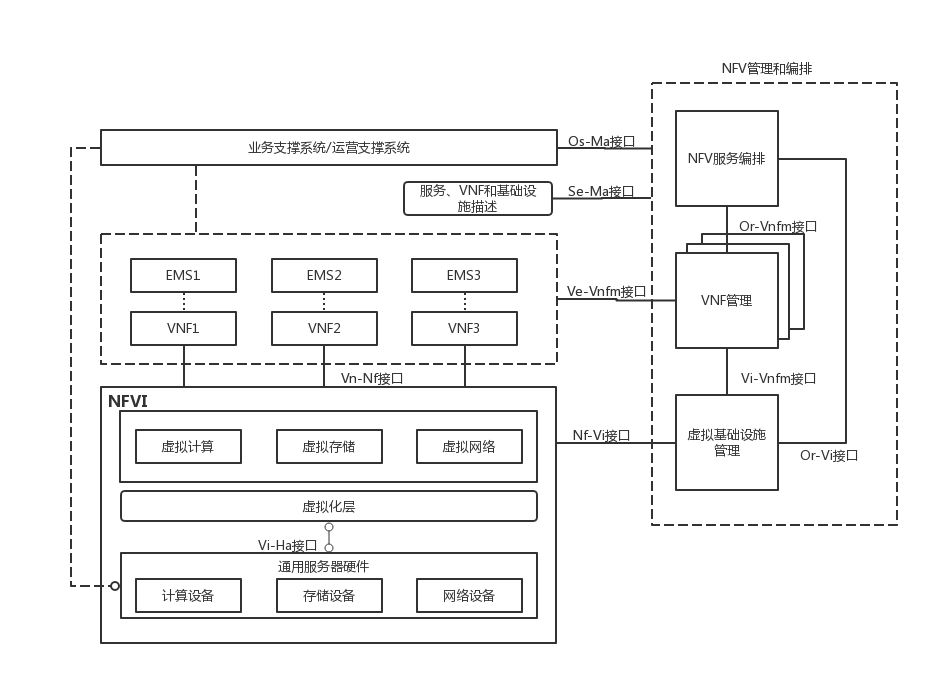
\includegraphics[width=1\textwidth]{ETSI.png}
	\bicaption[fig:NFV]{NFV标准框架}{NFV标准框架}{Fig}{NFV Standard Architecture}
\end{figure}

%为了实现NFV,保证NFV从专门的硬件中迁移到普通服务器中性能和资源分配管理是现阶段学术界和工业界所面对的主要问题\cite{mijumbi2016network}。根据已有的研究总结,当下的通用服务器要面对以下几个NFV环境下的新挑战\cite{hawilo2014nfv}:(1)通信网络中数据面的大负载而带来的性能压力。 (2)电信网络拓扑对管理的严格要求。这些挑战都亟待解决,并且对实现NFV功能落地具有重要意义。

在NFV的众多热点技术中,虚拟化资源调度作为NFV管理与编排系统的核心业务成为了工业界和学术界研究的热点问题。而其中的服务链技术 (SFC,Service Function Chain) 更是因为其接近实际应用场景的特点,受到广大研究的重点关注 \cite{zave2017dynamic,kulkarni2017nfvnice,mijumbi2016network} 。在传统网络中,负载均衡器、网关、虚拟防火墙等网络功能共同被称为业务功能点,而流量在经过了一系列处理后,形成了所谓的网络功能服务链。与虚拟化流量调度方式不同,该方式更倾向于对虚拟网络中如何通过控制服务器对网络流量转发进行编程控制,即以更为灵活的方式实现流量到业务功能点的调配和处理。在SFC中,网络的转发效率决定了整体网络的性能,所以如何优化虚拟化资源分配对于提升NFV性能具有重要意义。
	
学术界目前对于SFC的研究主要集中在两方面:(1)优化通用操作系统和网络协议栈,自底向上地提升NFV应用的性能,打破网络服务中来自底层通用平台和通用操作系统的性能瓶颈。(2)提出针对NFV应用的资源分配算法,优化资源分配效率和网络功能服务节点间网络流量的路径规划。

其中,在优化通用操作系统网络协议栈的方向,近些年学术界涌现了一系列的研究 \cite{rizzo2012netmap,ram2013hyper,belay2014ix,hwang2015netvm,yasukata2016stackmap,prekas2017zygos} ,结合工业界提出的高速网络包转发框架DPDK \cite{intel2015data} ,从简化网络协议栈,重新分配虚拟化资源和减少无关开销等角度尝试优化基于x86服务器的操作系统和虚拟化框架。这些方法都提高了标准通用服务器的网络性能,然而这些研究并未针对实际的NFV应用进行特定的优化,忽略了NFV应用的特有的各网络功能节点组织形式如服务链等,仍然从一般系统软件的角度去提升基础网络性能,针对NFV具体组织形式的底层优化仍然较少。

文献 \citen{xie2016service} 指出在NFV资源分配问题 (NFV resource allocation,NFV-RA) 中,如何解决基于NFV网络基础设施的资源分配是一项重要的挑战。进一步的,文献 \citen{herrera2016resource} 中将该问题划分为更细的粒度进行深入研究,为研究此类的问题指出了具体的研究方向。这类问题与文献 \citen{belbekkouche2012resource,fischer2013virtual} 所提出的传统网络中的网络功能映射问题 (Virtual Network Embedding,VNE) 相关,已有的研究参照VNE问题的研究成果和NFV背景下的具体问题,提出了一系列与实际应用相结合的启发式算法。有的从网络时延角度出发,如文献 \citen{mijumbi2015design} 所述,对NFV的部署和映射问题进行建模,给出了基于贪心和禁忌搜索的两种针对虚拟网络功能转发图映射和虚拟网络功能调度子问题的求解。此外,文献 \citen{lin2016demand} 从网络开销角度出发,提出了基于混合整数线性规划的方法来最小化网络功能的部署和网络流量的路由问题。这些研究都从上层角度结合NFV的应用给出了解决NFV实际应用的思路,但是大部分研究使用仿真的平台进行算法有效性的验证,对于求解问题实际物理平台上的可行性缺乏有力的证明。

\section{国内外研究现状}
\label{intro:research}
本节介绍并讨论与研究课题相关的国内外研究现状与发展趋势,重点包括国内外研究中对网络功能虚拟化中服务链问题的介绍,针对网络I/O优化,NFV资源分配问题,以及国内外研究者在多核架构下针对该问题的一些研究成果。同时,本章中也将本文所设计的优化解决方案与已有的解决方案和处理思路进行对比,对相关研究的研究内容进行比较和优缺点的分析。

\subsection{网络功能服务链}
根据文献 \citen{bhamare2016survey} 的定义,网络功能服务链是抽象服务功能 (Service Function,SF) 的有序或部分有序集合,包括对数据包,数据帧和数据流的有序约束分组。由于服务拓扑的复杂性,各个功能节点在服务链中的位置应具有相对的灵活性。文献 \citen{quinn2015problem} 总结了现阶段SFC研究所面临的挑战,主要包括:(1)复杂的网络拓扑依赖。原有的服务链是在硬件层面实现的,网络功能与底层硬件拓扑是绑定的,因此网络功能的增加与删减需要直接操作硬件,而NFV所带来的虚拟网络功能需要网络管理员最大可能的优化利用现有的网络资源,复杂的网络拓扑会给动态管理网络功能带来挑战。(2)严格的配置管理。服务链的网络功能节点顺序有着严格的要求,错误的服务配置会导致服务失败,严重影响服务质量,因此如何保证服务链的正确配置也是业界重点关注的领域 (3)受约束的服务弹性。服务链复杂的拓扑限制了服务链快速伸缩的弹性,服务链中任何一个网络节点的失效都可能导致服务链的伸缩失败,保证服务链所以功能节点的可用性对实现可扩展的服务链具有重要意义。文献 \citen{ghaznavi2015elastic} 研究了在弹性网络功能下的服务链放置问题,虽然与传统的网络放置问题相似,但网络功能额外的灵活有序要求对该类问题进行重新建模,并基于新的模型进行求解和优化。本文所研究的网络功能服务链是基于传统的串行服务链,针对服务链所运行的通用服务器平台资源进行建模并优化求解。相比于已有的研究,本文使用更接近实际应用平台的具体NFV业务,并借助虚拟化平台和具体业务平台来具体实现NFV业务,所得出的解决方法和结论更具有代表意义。

\subsection{网络I/O优化}
为了减小在虚拟化环境中运行虚拟机所带来的额外开销,文献 \citen{martins2014clickos} 对虚拟机操作系统进行了裁剪,使用微内核的方式构建了基于MiniOS \cite{popuri2014tour} 的最小化操作系统ClickOS,并在Xen \cite{barham2003xen} 的基础上将后端交换机Open vSwith \cite{pfaff2015design} 替换为了高速的VALE交换机 \cite{rizzo2012netmap} ,使用Click语言 \cite{kohler2000click} 进行NFV网络功能逻辑搭建,从而大大减少了虚拟化所带来的性能开销,提升了虚拟机的网络吞吐。但是在小包的测试环境中,该系统出现了剧烈的性能抖动,而且所能实现虚拟网络功能仍处于单个功能节点阶段,尚未组成服务链,并不能满足NFV复杂的业务需求。相比文献 \citen{martins2014clickos} ,文献 \citen{hwang2015netvm} 基于KVM平台 \cite{kivity2007kvm} 推出了NetVM,利用了高速的包转发框架DPDK \cite{intel2015data} 大大提升了网络协议栈的包转发速率,并通过共享大页内存、零拷贝数据传输以及优化CPU调度器提升了数据在VM之间的传输效率,减少了由于虚拟化中虚拟CPU的调度所引起的上下文切换开销。本文中借鉴了文献 \citen{hwang2015netvm} 的平台,在KVM基础上使用virtio \cite{russell2008virtio} 方式来优化VM之间的网络传输性能,通过优化多核服务器中虚拟机间资源的亲和度关系,解决在SFC的背景下NFV应用的性能优化问题。

文献 \citen{panda2016netbricks} 针对基于虚拟化技术实现的NFV提出不同的看法,认为基于现有的虚拟化技术 (VM或容器)所提供的隔离性会带来很高的性能开销,并且针对虚拟化来开发相应的网络功能是个十分繁琐的过程,为了减少这类与服务无关的开销,他们提出了一个新的NFV框架NetBricks来解决这两个问题。对于构建NF,文献 \citen{panda2016netbricks} 使用Rust语言构建了一小组可定制的网络处理元素,利用该语言的类型检查和安全运行机制来提供基于软件的隔离,将网络功能虚拟化与虚拟化框架解耦,使得软件化的网络功能不再依赖虚拟化平台,极大地减少了构建网络功能的开销,从而实现整体I/O性能的提升。文献 \citen{panda2016netbricks} 所提出的优化思路十分值得借鉴,但是现阶段完全抛开虚拟化框架实现NFV的成本太高,而且现有的虚拟化管理框架所带来的优势并不能体现,这样的做法会使得NFV失去与当前云计算平台相结合的优势。本文依然采用的是基于KVM的虚拟机实现模式,尽管虚拟化会引起较高的开销,但是同时所带来的更加简单的实现方式,以及更好的隔离性保障可以使得我们专注于解决服务链的资源分配问题。


\subsection{NFV资源分配问题}
在NFV资源分配问题方面,文献 \citen{herrera2016resource} 详细介绍了NFV资源分配问题的研究现状,总结了资源分配问题的具体子问题,即虚拟网络功能组链 (VNFs Chain Composition,VNFs-CC), 网络转发图映射 (VNF-Forwarding Graph Embedding,VNF-FGE)和虚拟网络功能调度 (VNFs Scheduling, VNFs-SCH)。文献 \citen{herrera2016resource} 将NFV下的资源分配问题归结为一类NP-Hard问题,并指出了解决此类问题的三种解法思路:确定解法、启发式解法和元启发式解法。具体来讲,针对VNF-FGE问题,确定解法中的整数线性规划方法可以在可接受的时间内给出最优解。而在时间敏感的NFV-RA问题下,确定解法的时间开销超出了预期限制,这时就需要借助基于启发式和元启发式的高级算法来减少算法的运行时间和额外开销。根据文献 \citen{herrera2016resource} 的归纳和总结,本文沿用了其解决该类问题的解法思路,使用基于贪心的确定解法来解决较小规模下的虚拟网络功能组链和映射问题。

文献 \citen{hsieh2016network} 认为在数据中心,网路功能服务链使工作流以特定的顺序遍历不同的网络功能,为客户提供不同级别的服务。由于服务链中任何相邻网络功能之间的距离将决定该链路的总带宽消耗,那么虚拟化网络功能在数据中心中的放置便成为了影响整体带宽的重要问题。在文献 \citen{hsieh2016network} 中,这种放置问题被归结为一个多重背包问题 (Multiple Knapsack Problem) 。文献 \citen{hsieh2016network} 针对树状网络拓扑,文章提出了两种基于贪心的算法:多层最差拟合和多层最佳拟合。在仿真平台的实验结果表明,与传统的最优算法相比,优化算法可以将带宽消耗降低15\%,而使用服务器数量仅增加1\%。文献 \citen{hsieh2016network} 使用组合优化的思想来归结此类问题可以使得问题变得更加清晰明了,但是算法仅在仿真平台上得到了验证,本文却利用真实的NFV应用平台对所提出的算法进行了验证,结论更具有说服力。


\subsection{其他相关研究}
除了对于网络I/O的优化和NFV资源分配问题的研究,很多文献和论文也从其他角度如MANO系统和操作系统线程等方面,对网络功能虚拟化进行了研究。

文献 \citen{mijumbi2016management} 总结了在网络功能虚拟化管理和编排时可能会遇到的挑战。文章结合虚拟化所带来的资源体量的增加,分析了如何在现有的庞大的基础设施中获取有效的产出所需要面对三个主要问题:(1) NFV服务点 (Points of Presence, PoP) 的地理分布,为了更好地服务用户,如何确定虚拟网络功能集群的服务点地里位置对于电信运营商来说是重点挑战之一。严格的服务质量要求按照一定的最优化问题的方法来合理部署NFV服务的存在点,从而使得NFV服务可以保证覆盖所有服务范围。(2)虚拟网络功能放置,网络功能虚拟化是以一定逻辑链接的虚拟网络功能所组成的,服务链就是一种典型的组成形式,在NFV服务点中如何去合理部署具体的虚拟网络功能对于MANO框架来说具有重要意义。(3)动态资源管理,NFV服务的弹性需求要求MANO系统同样能够支持动态地分配和调度物理资源以实现服务链的伸缩目标,能够满足不同需求规模下的服务实现。

文献 \citen{hu2016towards} 认为当前在使用NFV部署在现代的大通量标准服务器时会面临许多挑战。因为NFV数据平面及其服务功能链的复杂性特征,现代NFV应用以异构软件流水线的方式部署在大容量通用服务器上。文献 \citen{hu2016towards} 从操作系统运行线程的角度出发,考虑到NFV应用流量必须由异构处理软件从网卡到终端接收器。由于流程的端到端性能是由每个处理阶段的性能共同决定的。基于底层物理架构的的大容量通用服务器中的资源分配映射方案必须考虑线程间的依赖调度来减少资源竞争所带来的影响。在文献 \citen{hu2016towards} 中,他们提出了一个可以协同放置最小化端到端访问开销的线程调度机制来调度异构的软件线程来最小化NFV线程应用线程端到端的数据传递开销。为了更加方便地评估各线程的数据传递开销,文献 \citen{hu2016towards} 还提出了一个基于线程资源的NFV应用性能下降模型,通过这个模型来衡量数据异构的软件流水线中传递时所造成的开销。本文相比于文献 \citen{hu2016towards} ,更加侧重于考虑虚拟化所造成的影响,虽然从主机的角度来看,虚拟机也是以线程方式运行在主机上,但是虚拟机软件栈会屏蔽虚拟机内部应用的具体信息,而且现有的基于虚拟机的I/O虚拟化技术也会对虚拟机线程间的数据传递有重要影响,本文结合virtio的I/O虚拟化方式,从虚拟机的角度来解决NFV应用的资源分配问题,从而提高NFV应用的整体性能。

\section{论文安排}
本文对网络功能虚拟化中,虚拟机资源调度进行了研究,论文的具体结构和内容安排如下:

第一章作为绪论,主要介绍了本课题的主要研究内容和研究背景。进一步的对于本研究相关的工作进行了介绍和梳理,主要从网络I/O优化研究和NFV资源分配研究两个角度以及其他相关研究介绍了国内外已有的研究成果。最后本章对全文的结构和安排做了介绍。

第二章重点介绍了与本文的研究紧密相关的研究背景和相关技术,包括NFV的发展历程,目前主流的网络I/O虚拟化技术分类,多核服务器架构已经在多核服务器下的虚拟机性能观测,最后还介绍了本文所使用的NFV应用平台Clearwater,为读者了解与研究相关的知识和下文的展开做了准备。

第三章着重介绍了本研究中研究方案的具体设计,包括方案的设计目标,基于服务链的建模,系统的设计思路和系统具体的模块设计等。同时,也依次详细介绍了文本的设计方案的各个子模块的具体设计思路,描述了基于模块设计的系统工作流。

第四章将介绍本研究中的研究方案的具体实现,以总体算法框架为切入点,分模块介绍了本文系统各子模块的实现方法。

第五章从实验的角度对本文的设计进行了性能上的测试。通过利用Clearwater自带的压力测试工具和基础性能测试工具iPerf、Ping、Apache等,在真实的测试环境下对本文所提出的系统进行了严格的测试。

第六章归纳全文,总结和回顾了全文的研究内容和主要研究结论,并提出了一些研究展望。

\section{本章小结}
本章主要整理和归纳与本研究密切相关的国内外研究现状和发展趋势。本章中,重点介绍了国内外的相关研究中,网络功能虚拟化带来的一系列挑战和存在的问题。同时,本章中也对现有解决方案进行了深入的探讨,分析这些方案的共同点和优缺点,与本研究中的设计相对比。本章也对网络功能虚拟化的研究热点进行了介绍,特别是对当前研究较为火热的资源调度问题及相关研究的研究成果进行了简单的归纳和总结。